\documentclass[class=article,border=5pt,tikz]{standalone}
\usetikzlibrary{intersections,backgrounds}

\usetikzlibrary{calc}

% Define all coordinates
\tikzset{
  define coordinates/.style={
    execute at begin picture={
      \def\a{1}
      \def\b{0.7}
      \coordinate (O) at (0,0);
      \coordinate (A) at (-\a/2,\a/2);
      \coordinate (B) at (\a/2,\a/2);
      \coordinate (C) at (\a/2,-\a/2);
      \coordinate (D) at (-\a/2,-\a/2);
      \coordinate (E) at (-\b/2,\b/2);
      \coordinate (F) at (\b/2,\b/2);
      \coordinate (G) at (\b/2,-\b/2);
      \coordinate (H) at (-\b/2,-\b/2);
   }
 },
every picture/.append style={define coordinates} % will apply this to all tikzpictures
}


\begin{document}

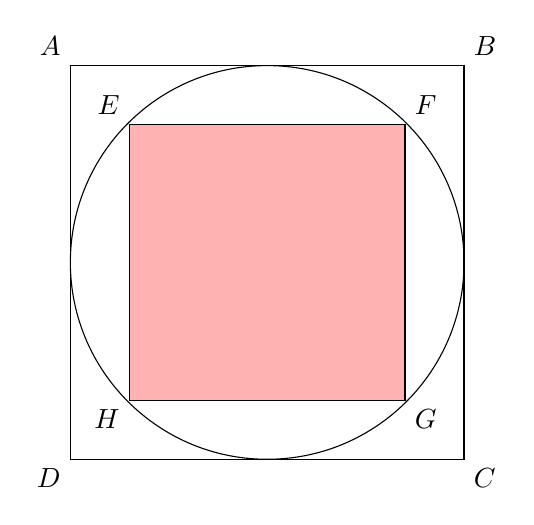
\begin{tikzpicture}[scale=5]

% Draw the main square and labels
\draw (A) node [above left]  {$A$} -- 
      (B) node [above right] {$B$} -- 
      (C) node [below right] {$C$} -- 
      (D) node [below left]  {$D$} -- 
          cycle;

% Draw the inscribed square and labels
\draw (E) node [above left]  {$E$} -- 
      (F) node [above right] {$F$} -- 
      (G) node [below right] {$G$} -- 
      (H) node [below left]  {$H$} -- 
          cycle;

% Draw the inscribed circle
\draw (O) circle (0.5*\a cm);

% fill the inscribed square
\begin{pgfonlayer}{background}% background otherwise it 'leaks'
  \fill [color=red,opacity=0.3] (E) -- (F) -- (G) -- (H) -- cycle;
\end{pgfonlayer}

\end{tikzpicture}


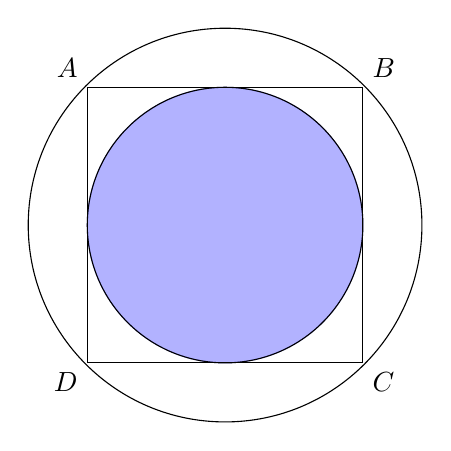
\begin{tikzpicture}[scale=5]

% Draw the inscribed square and labels
\draw (E) node [above left]  {$A$} -- 
      (F) node [above right] {$B$} -- 
      (G) node [below right] {$C$} -- 
      (H) node [below left]  {$D$} -- 
          cycle;

% Draw the main circle
\draw (O) circle (0.5*\b cm);

% Draw the inscribed circle
\draw (O) circle (0.5*\a cm);

\begin{pgfonlayer}{background}% background otherwise it 'leaks'
  \filldraw [color=blue,opacity=0.3] (O) circle (0.5*\b cm);
\end{pgfonlayer}

\end{tikzpicture}

\end{document}
